% XSuM-MicroBooNE technote. Build: bash docs/technote/build.sh (needs pdflatex; the schematic is docs/technote/schematic/).
\documentclass[10pt,letterpaper]{article}
\usepackage[margin=22mm]{geometry}
\usepackage[T1]{fontenc}
\usepackage{lmodern}
\usepackage{amsmath,amssymb}
\usepackage{booktabs,longtable,array,multirow}
\usepackage{graphicx}
\usepackage{rotating,float}
\usepackage{xcolor}
\usepackage{enumitem}
\usepackage[hidelinks]{hyperref}
\usepackage{url}
\urlstyle{tt}
\setlength{\parskip}{3pt plus 1pt}
\newcommand{\code}[1]{\texttt{#1}}
\newcommand{\pct}[1]{#1\%}
\definecolor{cdone}{HTML}{009E73}\definecolor{cpart}{HTML}{E69F00}\definecolor{cmiss}{HTML}{8C8C8C}
\newcommand{\sdone}{\textcolor{cdone}{\textbf{done}}}
\newcommand{\spart}{\textcolor{cpart}{\textbf{defined}}}
\newcommand{\smiss}{\textcolor{cmiss}{\textbf{not started}}}

\title{XSuM-MicroBooNE: a surrogate detector model for the MicroBooNE open sample\\[2mm]
  \large Technote 1: the sample, what it gives a surrogate, and the plan}
\author{Linyan Wan\\ \small Fermi National Accelerator Laboratory}
\date{18 November 2026}

\begin{document}
\maketitle

\begin{abstract}
\noindent
XSuM-MINERvA is a generative surrogate of the MINERvA detector trained on the MINERvA open dataset: it maps the
final-state particles of a simulated interaction to the reconstructed quantities of the analysis tuples, so that events
from any generator can be run through it. This note starts the same programme on MicroBooNE's open samples, for the
\emph{BNB inclusive overlay sample without wire information} (Zenodo record 8370883: 18 HDF5 files, 195\,GB,
753\,467 events). It records what the files contain, what was measured on the first file without downloading it, how
the truth and reconstruction sides are slimmed, where the MicroBooNE case differs from the MINERvA one, and, on a
schematic of the full chain, which steps exist and which are missing. The main findings: the reconstruction in the HDF5
files stops at Pandora's pattern recognition (a neutrino slice, its vertex and scores, its PFParticles with a
track/shower score) with no track fits, calorimetry or particle identification; the Geant4 primaries carry no direction;
and the files carry no exposure. The surrogate's output is therefore the Pandora level, per-PFParticle charge and extent
must be derived from the hit tables, and directions and POT must come from the artroot files. Repository:
\url{https://github.com/linyan-w/XSuM-MicroBooNE}.
\end{abstract}

\tableofcontents

\section{Purpose and scope}

The MINERvA surrogate (XSuM-MINERvA, \url{https://github.com/linyan-w/XSuM-MINERvA}) takes one event of generator
truth (vertex, nucleus, post-FSI particle list) and returns a reconstructed event in the open dataset's format, drawn
from a conditional generative model trained on the open dataset's own (truth, reconstruction) pairs; an ensemble of
trainings gives the model uncertainty as systematic universes. The aim here is the same model class for MicroBooNE,
trained on the open sample MicroBooNE released for exactly this kind of collaborative development
\cite{cerati2023}. The first step is to understand what the open sample is and what it can teach a surrogate, which
is what this note does. The schematic in Figure~\ref{fig:schematic} and Section~\ref{sec:status} say where the work
stands.

Nothing of the sample is stored locally: every measurement here was made by reading the first file in place from
Zenodo over HTTP range requests (metadata and the first chunks of each column, a few tens of MB), because the machine
has about 30\,GB free and one file is 11\,GB. A fetch script with a disk reserve exists for when a file is needed.

\section{The open sample}\label{sec:sample}

MicroBooNE's \emph{BNB Inclusive Overlay Sample (No Wire Info)}, Zenodo record
\href{https://doi.org/10.5281/zenodo.8370883}{10.5281/zenodo.8370883}, version ``large'' (2023-09-26), CC~BY~4.0
\cite{zenodo8370883}: simulated Booster Neutrino Beam interactions of every flavour and interaction type, with the
relative abundances of the nominal flux and cross-section models, generated in the whole cryostat and overlaid on
beam-off data of the detector, i.e.\ real cosmic rays and noise. Documentation and example notebooks are in
\url{https://github.com/uboone/OpenSamples} (tag v02) \cite{opensamples}; the collaboration's column-by-column
description is reproduced in Appendix~\ref{app:content}. One HDF5 ``event'' is one detector readout with one
simulated neutrino interaction plus the overlaid cosmic activity.

\begin{table}[H]\centering\small
\caption{The record. The sizes are from the Zenodo API; the manifest with every file's size, md5 and URL is
\code{configs/zenodo\_8370883\_files.txt} in the repository.}\label{tab:record}
\begin{tabular}{@{}p{70mm}rrp{45mm}@{}}\toprule
content & files & size & events\\ \midrule
\code{BNB\_All\_NoWire\_00.h5} \ldots\ \code{\_17.h5} & 18 & 194.9\,GB & 753\,467 (42\,674 in file 00)\\
\code{public-artroot-bnb-all.list}: xrootd URLs of the artroot files & 1 & 8.5\,MB & 1\,046\,139 in 24\,436 files, 6.4\,TB\\
\bottomrule\end{tabular}
\end{table}

The ``NoWire'' files omit the wire waveforms, which dominated the file size, so that more events fit: the companion
``WithWire'' inclusive sample has 24\,332 events. The electron-neutrino samples (89\,339 events NoWire) are separate
records.

\paragraph{What is not in the files.} There is no generator-level record beyond the event table (flavour, energy,
direction, CC/NC, lepton energy, vertex): no interaction mode, no initial-state nucleon, no event weight. There is no
exposure (POT) in the files or on the record. The generator (GENIE in MicroBooNE's MCC9 configuration), the flux and
the POT are in the artroot files and the collaboration's documentation and must be taken from there.

\section{Content of the HDF5 files}\label{sec:content}

Every table is a group of column datasets with one row per object, plus an auxiliary dataset
\code{event\_id.seq\_cnt} of rows \code{[event\_seq, count]}: for each event that has rows in the table, the event's
position in \code{event\_table} and its number of rows, in file order. Rows of one event are contiguous, so a table can
be read for a range of events with one slice per column; this is what \code{xsum.io.h5.Sample} does, locally or over
HTTP. Table~\ref{tab:tables} lists the tables of file 00 with their sizes; the column meanings are in
Appendix~\ref{app:content}.

\begin{table}[H]\centering\footnotesize
\caption{Tables of \code{BNB\_All\_NoWire\_00.h5} (42\,674 events). ``Events'' is the number of events with at least one
row. Vector columns carry their width in brackets.}\label{tab:tables}
\begin{tabular}{@{}lrrp{95mm}@{}}\toprule
table & rows & events & columns\\ \midrule
\code{event\_table} & 42\,674 & 42\,674 & event\_id[3], is\_cc, lep\_energy, nu\_dir[3], nu\_energy, nu\_pdg, nu\_vtx[3], nu\_vtx\_corr[3], nu\_vtx\_wire\_pos[3], nu\_vtx\_wire\_time\\
\code{particle\_table} & 4\,011\,145 & 35\,430 & g4\_id, g4\_pdg, parent\_id, momentum, category, instance, start/end\_process, start/end\_position[3], start/end\_position\_corr[3], start/end\_wire\_pos[3], start/end\_wire\_time\\
\code{edep\_table} & 40\,439\,430 & 35\,430 & energy, energy\_fraction, g4\_id, hit\_id\\
\code{hit\_table} & 674\,335\,781 & 42\,674 & hit\_id, integral, local\_plane, local\_time, local\_wire, rms, tpc\\
\code{pandoraHit\_table} & 674\,335\,781 & 42\,674 & hit\_id, pfp\_id, slice\_id\\
\code{pandoraPrimary\_table} & 1\,352\,085 & 42\,674 & slice\_id, slice\_pdg, nu\_score, flashmatch\_score, vtx[3], vtx\_wire\_pos[3], vtx\_wire\_time\\
\code{pandoraPfp\_table} & 45\,068 & 18\,375 & pfp\_id, pfp\_pdg, trkshr\_score, vtx[3], vtx\_wire\_pos[3], vtx\_wire\_time\\
\code{opflash\_table} & 42\,059 & 36\,900 & flash\_id, time, time\_width, totalpe, wire\_pos[3], y\_center, y\_width, z\_center, z\_width\\
\code{opflashsumpe\_table} & 1\,027\,947 & 36\,900 & flash\_id, pmt\_channel, sumpe, sumpe\_id\\
\code{ophit\_table} & 15\,317\,703 & 42\,674 & hit\_id, hit\_channel, pe, peaktime, width, amplitude, area, sumpe\_id, wire\_pos[3]\\
\bottomrule\end{tabular}
\end{table}

\paragraph{Truth side.} \code{event\_table} holds the interaction: \code{nu\_pdg}, \code{nu\_energy}, \code{nu\_dir},
\code{is\_cc}, \code{lep\_energy}, the true vertex \code{nu\_vtx} and the space-charge-corrected vertex
\code{nu\_vtx\_corr}, which is the one to compare with the reconstruction. \code{particle\_table} holds the Geant4
particles; the rows with \code{start\_process == "primary"} (parent 0) are the particles that emerge from the
neutrino interaction, i.e.\ the generator's final state after final-state interactions as handed to Geant4, and are the
surrogate's input. The table stores the momentum magnitude and the start and end positions, not the momentum vector.
\code{edep\_table} links energy deposits to hits and particles: the hit-level ground truth, not needed by a surrogate.

\paragraph{Reconstruction side.} \code{pandoraPrimary\_table} lists every Pandora slice of the readout (about 30 per
event, almost all cosmic, \code{slice\_pdg}~=~13). The slice with \code{slice\_pdg} 12 or 14 is Pandora's neutrino
candidate: there is at most one per event, with its vertex, \code{nu\_score} and \code{flashmatch\_score}.
\code{pandoraPfp\_table} holds the PFParticles of the neutrino candidate only: track-like (\code{pfp\_pdg}~13) or
shower-like (11), the \code{trkshr\_score} and the start point. The hits (\code{hit\_table}: integral in ADC, plane,
wire, time) and their assignment to PFParticles and slices (\code{pandoraHit\_table}) are there, about 16\,000 per
event, but nothing downstream of pattern recognition: no track fits, no calorimetric energies, no particle-identification
scores, no event-level kinematics. The optical tables give the flashes; the beam-window flash (3--5\,$\mu$s) and its PE
and barycentre are the ones that matter.

\paragraph{Undocumented values.} \code{slice\_pdg}~=~11 occurs (721 of 63\,152 slices in 2\,000 events), is not in the
collaboration's description, \pct{88} of those rows have vertex $-999$, and such a row never is the neutrino candidate;
they are ignored. Rows of \code{pandoraPrimary\_table} with \code{nu\_score}~=~$-999$ (cosmic slices without a score)
and \code{flashmatch\_score}~=~9999 (no match attempted) are sentinels.

\section{Measured properties of the sample}\label{sec:measured}

Measured on the first 2\,000 events of file 00 with \code{scripts/curate/h5\_summary.py} (2026-11-03). They are design
guides, not final numbers.

\begin{table}[H]\centering\small
\caption{The interaction (event table).}\label{tab:event}
\begin{tabular}{@{}>{\raggedright\arraybackslash}p{52mm}p{108mm}@{}}\toprule
flavour & $\nu_\mu$ 0.981, $\bar\nu_\mu$ 0.007, $\nu_e$ 0.011, $\bar\nu_e$ 0.001\\
charged current & 0.709\\
$E_\nu$ (GeV), p50/90/99 & 1.09 / 1.76 / 4.23; lepton energy 0.56 / 1.22 / 2.82\\
true vertex in the active volume & 0.419 (the sample is generated in the whole cryostat)\\
vertex range (cm) & $x$ $-63$ to 319 (p50 133), $y$ $-191$ to 191 (p50 $-2$), $z$ $-82$ to 1118 (p50 508)\\
space-charge shift $|\vec v_\text{corr}-\vec v|$ (cm), p50 / p99 & $x$ 1.1 / 4.6, $y$ 0.03 / 11.0, $z$ 0.003 / 3.5\\
grouping & 29 runs, 120 subruns in the 2\,000 events\\
\bottomrule\end{tabular}
\end{table}

\begin{table}[H]\centering\small
\caption{The Geant4 primaries (particle table). ``Selected'' means above 10\,MeV kinetic energy with the outgoing
neutrino of NC events dropped and neutrons kept.}\label{tab:particles}
\begin{tabular}{@{}>{\raggedright\arraybackslash}p{52mm}p{108mm}@{}}\toprule
particle rows per event, p50/90/99 & 40 / 224 / 717; primaries 2 / 6 / 22\\
primary PDG counts (2\,000 events) & $n$ 2406, $p$ 2166, $\mu^-$ 850, $\pi^+$ 243, $\pi^0$ 221, $\pi^-$ 103, $e^-$ 14, $\gamma$ 7, $\mu^+$ 4, $K^\pm$ 3, $^{40}$Ar 1\\
selected primaries per event, p50/90/99/max & 2 / 5 / 14 / 22\\
selected by model class & $n$ 1864, $p$ 1702, $\mu^-$ 847, $\pi^+$ 241, $\pi^0$ 217, $\pi^-$ 101, $e^-$ 14, $\gamma$ 6, $\mu^+$ 4, $K^\pm$ 3, other 1\\
primaries with coincident start and end & 0.018 (no direction proxy)\\
events with no particle rows at all & 0.17 (all with the vertex outside the active volume, most of them CC): Geant4 particles are recorded only when the products reach the TPC region\\
\bottomrule\end{tabular}
\end{table}

\begin{table}[H]\centering\small
\caption{Pandora and the optical system.}\label{tab:pandora}
\begin{tabular}{@{}>{\raggedright\arraybackslash}p{52mm}p{108mm}@{}}\toprule
slices per event, p50/90/99 & 30 / 43 / 62; \code{slice\_pdg} counts: 13 (cosmic) 61\,647, 14 ($\nu_\mu$) 705, 12 ($\nu_e$) 79, 11 (undocumented) 721\\
events with a neutrino slice & 0.392 overall; 0.657 with the true vertex in the active volume, 0.201 outside\\
$\nu$ score of the neutrino slice, p10/50/90 & 0.011 / 0.32 / 0.99; flash-match score p50/90: 5.1 / 52\\
slices with any $\nu$ score & 0.411; with a flash-match score 0.436\\
$|\vec v_\text{slice}-\vec v_\text{corr}|$ (cm), p50/90/99 & 4.6 / 197 / 336 (all); 0.73 / 123 / 312 (vertex in the active volume); per axis p50 inside: 0.2, 0.4, 0.4\\
PFParticles of the neutrino slice, p50/90/99/max & 2 / 4 / 6 / 10; never zero when a slice exists\\
\code{pfp\_pdg} & 13 (track) 1482, 11 (shower) 355; \code{trkshr\_score} p10/50/90: 0.06 / 0.93 / 1.0\\
flashes per event, p50/90/99 & 1 / 2 / 2; events without a flash 0.151\\
flash time ($\mu$s), p1/50/99 & 2.6 / 4.5 / 22.6; total PE p50/90/99: 697 / 4153 / 9413\\
\bottomrule\end{tabular}
\end{table}

Two things stand out. The ``reconstructed'' flag of this sample, a neutrino slice exists, is \pct{66} inside the active
volume and \pct{20} outside it; the outside ones are cosmic slices that Pandora labelled as the neutrino, with vertices
far from the truth (the long tail of the vertex residual). And the resolution of the slice vertex on the correct slice
is a few millimetres per axis, an order of magnitude better than MINERvA's, so the vertex column of an event flow will
be a narrow core with a wide wrong-slice tail: a mixture that wants its own class, as the vertex-plane head had in
MINERvA.

\section{Differences from the MINERvA case}\label{sec:diff}

Table~\ref{tab:diff} sets the two cases side by side. The MicroBooNE input is poorer (no direction, no interaction
mode, no exposure) and its reconstruction output is at an earlier stage (pattern recognition rather than fitted tracks
and calorimetry), but it is also simpler: one flag, one vertex, a handful of PFParticles, and a far larger cosmic
component that the surrogate inherits from the overlay for free.

\begin{table}[H]\centering\footnotesize
\caption{What shapes the design, side by side.}\label{tab:diff}
\begin{tabular}{@{}p{24mm}p{58mm}p{80mm}@{}}\toprule
 & MINERvA (XSuM-MINERvA) & MicroBooNE (this work)\\ \midrule
input particles & \code{mc\_FSPart*}: species and three-momentum of every post-FSI particle & Geant4 primaries: species, $|\vec p|$, start and end position. No direction: the start-to-end displacement is the proxy, exact for particles that stop or leave without scattering, approximate otherwise; \pct{1.8} have no displacement\\
vertex & \code{mc\_vtx} (mm) & \code{nu\_vtx} and \code{nu\_vtx\_corr} (cm); space charge shifts $x$ by about 1\,cm (p50), up to 5--11\,cm\\
population & CC $\nu_\mu$ (later all events) in the inner detector, $z$ 4000--8700\,mm & every flavour; the active volume holds \pct{42} of the vertices, the rest is cryostat and is reconstructed only as a wrong slice. \pct{98} $\nu_\mu$, \pct{71} CC\\
reconstructed flag & a muon candidate exists (\pct{32} of Truth events) & a neutrino slice exists (\pct{39}; \pct{66} inside the active volume)\\
reco vertex & \code{MasterAnaDev\_vtx}, 10\,mm ($x,y$) and 40\,mm ($z$) & slice vertex, 2--4\,mm per axis (p50) with a wrong-slice tail (p90 123\,cm inside the volume)\\
muon & momentum, angle, MINOS match, charge & nothing muon-specific; PFParticles with a track score; momentum by range or multiple scattering is not in the files\\
calorimetry & three recoil energies & hit integrals (ADC) per PFParticle and plane, to be derived from the hit tables\\
prongs & up to 10 hadron prongs with pion and proton fits & 1--10 PFParticles (p50 2, p90 4) with a track/shower score and a start point\\
detector conditions & overlay dead time & overlay cosmics (about 30 cosmic slices per readout), the beam flash\\
exposure & \code{Meta/POT\_Used} per file & not in the files\\
units & MeV, mm & GeV, cm, ticks\\
\bottomrule\end{tabular}
\end{table}

\section{The surrogate: input, output, and where the work stands}\label{sec:status}

\begin{sidewaysfigure}[p]\centering
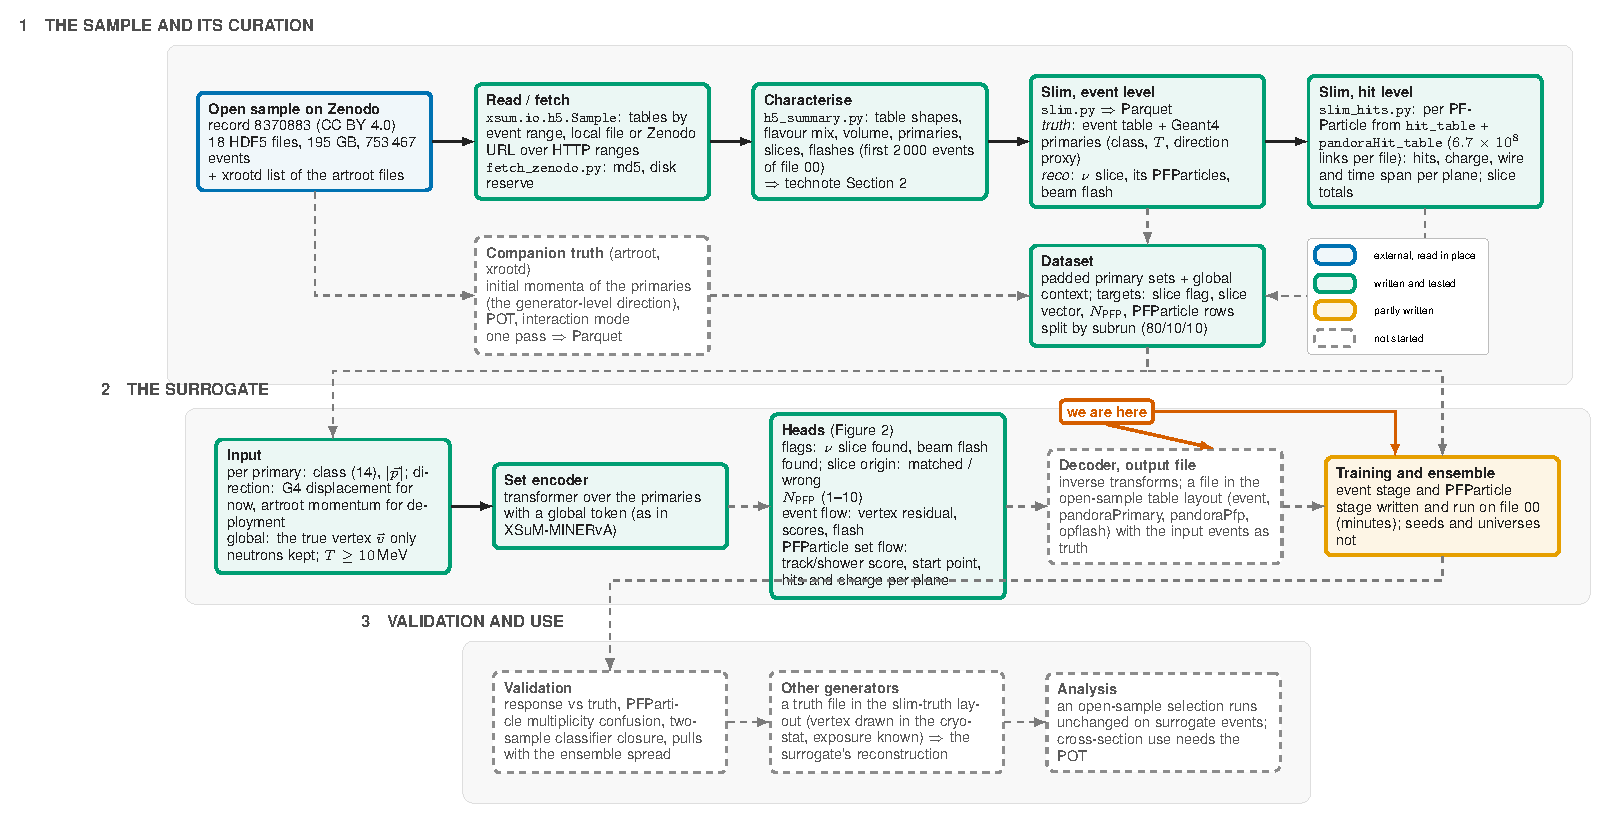
\includegraphics[width=\textheight]{schematic/schematic.pdf}
\caption{The chain from the open sample to an analysis on surrogate events, with the status of every step on
18 November 2026. Band 1 is the sample and its curation, band 2 the model, band 3 its validation and use. Green boxes
are written and tested in the repository, the orange one is defined on paper only, dashed boxes are not started; the
blue box is the external sample, read in place.}\label{fig:schematic}
\end{sidewaysfigure}

\paragraph{Input} (one event): $\vec v_\text{corr}$, \code{nu\_pdg}, \code{is\_cc}, $E_\nu$, and the set of primaries
above 10\,MeV kinetic energy with the outgoing neutrino of NC events dropped: class (14 classes,
\code{xsum.constants.CLASS\_NAMES}), kinetic energy and direction proxy. Neutrons are kept (they are the most common
primary) and so are events outside the active volume and events with no primaries at all, which are Truth-only events
with an empty input set. The slim truth file (\code{scripts/curate/slim.py}) holds exactly this plus the event
identifiers and an \code{in\_active\_volume} flag.

\paragraph{Output} (one event):
\begin{enumerate}[nosep]
\item \code{has\_nu\_slice} (Bernoulli): Pandora selected a neutrino slice.
\item Given a slice: its vertex (3), \code{nu\_score}, \code{flashmatch\_score}, \code{slice\_pdg} (12 or 14), the
  beam-flash PE and $y/z$ barycentre, and the number of PFParticles.
\item Per PFParticle: \code{trkshr\_score}, start point, and the hit-derived summary (charge per plane, hit count,
  extent along the direction, end point) once the hit tables are curated.
\end{enumerate}
The slim reco file holds items 1 and 2 and the PFParticle columns of the HDF5 file; the hit-derived columns are the
next curation step. The model can then follow XSuM-MINERvA: a set encoder on the primaries with the vertex and flavour
in the global token, Bernoulli heads for the flags, a categorical head for the number of PFParticles, an event flow for
the slice-level continuous quantities and a prong set flow for the PFParticles, with an ensemble of seeds for the model
uncertainty and the output written in the open sample's own table layout so that a selection written for the sample
runs unchanged.

\paragraph{Where we are.} Reading the schematic from the top left:
\begin{description}[nosep, leftmargin=28mm, style=sameline]
\item[\sdone] the sample is reachable in place (\code{xsum.io.h5.Sample}, local or over HTTP), with a manifest and a
  guarded fetcher (\code{fetch\_zenodo.py}); its structure and statistics are measured (\code{h5\_summary.py},
  Sections~\ref{sec:content}--\ref{sec:measured}); the event-level slimming into truth and reco Parquet is written
  (\code{slim.py}) and tested on a 300-event extract of file 00 (\code{tests/}, seven tests).
\item[\spart] the model input and output are defined (above), nothing more.
\item[\smiss] the hit-level slimming (per-PFParticle charge and extent from $6.7\times10^8$ hit links per file, one
  file at a time), the companion truth from the artroot files (directions, POT, interaction mode), the training
  dataset and split, the model and its training chain, the decoder and output file, the validation suite, and the
  path for other generators.
\end{description}

\section{Open questions}\label{sec:open}

\begin{enumerate}[nosep]
\item \textbf{Direction of the primaries.} Whether the start-to-end proxy is good enough, or whether the artroot
  \code{MCTruth}/\code{MCParticle} momenta must be extracted once (one pass over the artroot files via xrootd) and
  distributed as a companion truth file. The artroot file list is in the record.
\item \textbf{Exposure.} A POT per file, or a per-event weight, is needed for any cross-section use; it is not in the
  HDF5 files.
\item \textbf{Hit-level targets.} Which per-PFParticle quantities to derive from the hit tables, and the disk budget for
  doing so: 11\,GB per file, streamed one at a time.
\item \textbf{Wrong-slice events.} The \pct{20} of out-of-volume events with a ``neutrino'' slice are cosmic slices.
  The surrogate must either model them (a wrong-slice class with a vertex drawn from the cosmic distribution) or be
  restricted to the active volume; inside the volume the same tail exists at a lower rate.
\item \textbf{Split.} Events are grouped by run and subrun (120 subruns in 2\,000 events); split by subrun as in MINERvA
  so that overlay-correlated readouts stay together.
\end{enumerate}

\section{Repository and reproduction}\label{sec:repo}

\url{https://github.com/linyan-w/XSuM-MicroBooNE}, Apache 2.0 for the code; the data are the MicroBooNE
Collaboration's under CC~BY~4.0 \cite{zenodo8370883,microboone2017}.

\begin{table}[H]\centering\small
\begin{tabular}{@{}p{26mm}p{118mm}@{}}\toprule
\code{xsum/} & \code{io/h5.py} the reader, \code{io/tables.py} the columns used, \code{prep/} primaries and volume, \code{constants.py} conventions\\
\code{scripts/curate/} & \code{fetch\_zenodo.py}, \code{h5\_summary.py}, \code{slim.py}, \code{make\_example.py}\\
\code{configs/} & the Zenodo manifest (names, sizes, md5s, URLs)\\
\code{docs/technote/} & this note (\code{technote.tex}, \code{technote.pdf}), the schematic (\code{schematic/}), the collaboration's column documentation (\code{h5\_content.md}) and its converter\\
\code{tests/} & reader, preparation and slimming tests on the 300-event extract \code{tests/data/}\allowbreak\code{BNB\_All\_NoWire\_00.first300.h5} (2.3\,MB)\\
\bottomrule\end{tabular}
\end{table}

\begin{verbatim}
bash scripts/setup_env.sh && source .venv/bin/activate && pytest -q
python scripts/curate/h5_summary.py \
    "https://zenodo.org/api/records/8370883/files/BNB_All_NoWire_00.h5/content" --events 2000
python scripts/curate/fetch_zenodo.py data/h5 --files 00 --reserve-gb 20  # 11 GB, md5
python scripts/curate/slim.py data/h5/BNB_All_NoWire_00.h5 data/slim/BNB_All_NoWire_00
bash docs/technote/build.sh                                             # this note
\end{verbatim}

\begin{thebibliography}{9}
\bibitem{zenodo8370883} MicroBooNE Collaboration, \emph{MicroBooNE BNB Inclusive Overlay Sample (No Wire Info)},
  Zenodo (2023), \href{https://doi.org/10.5281/zenodo.8370883}{doi:10.5281/zenodo.8370883}.
\bibitem{opensamples} MicroBooNE Collaboration, \emph{OpenSamples: documentation and tutorials for accessing MicroBooNE
  open samples}, \url{https://github.com/uboone/OpenSamples}, tag v02.
\bibitem{cerati2023} G.~Cerati for the MicroBooNE Collaboration, \emph{MicroBooNE Public Data Sets: a Collaborative
  Tool for LArTPC Software Development}, CHEP 2023, \href{https://arxiv.org/abs/2309.15362}{arXiv:2309.15362}.
\bibitem{microboone2017} MicroBooNE Collaboration, \emph{Design and construction of the MicroBooNE detector},
  JINST 12 (2017) P02017.
\end{thebibliography}

\clearpage
\appendix
\section{Column documentation of the HDF5 files}\label{app:content}
\footnotesize
\begin{longtable}{@{}p{34mm}p{10mm}p{7mm}p{100mm}@{}}
\caption{Content of the open-sample HDF5 files, as documented by the collaboration (uboone/OpenSamples v02, \texttt{file-content-hdf5.md}; the \texttt{\#CHECK} marks are theirs). The \texttt{wire\_table} is absent from the NoWire files.}\label{tab:h5content}\\
\toprule entry & type & $n$ & description\\ \midrule \endfirsthead
\toprule entry & type & $n$ & description\\ \midrule \endhead
\bottomrule \endfoot
\addlinespace[3pt]\multicolumn{4}{@{}p{151mm}@{}}{\textbf{\texttt{/}} \quad Main entry point of the file.}\\
\addlinespace[3pt]\multicolumn{4}{@{}p{151mm}@{}}{\textbf{\texttt{/event\_table}} \quad Table storing information about a single detector readout and a single simulated neutrino interaction.}\\
\quad\texttt{event\_id} & dataset & 3 & Run/Subrun/Event number for a detector readout.\\
\quad\texttt{event\_id.seq\_cnt} & dataset & 2 & Auxiliary information added in post-processing step for simple grouping and fast access of table entries separated by event.\\
\quad\texttt{is\_cc} & dataset & 1 & If 1 the simulated neutrino interaction is charged-current, if 0 it is neutral-current.\\
\quad\texttt{lep\_energy} & dataset & 1 & Simulated energy of the lepton outgoing from the neutrino interaction (in GeV).\\
\quad\texttt{nu\_dir} & dataset & 3 & Initial direction of the simulated neutrino interacting in the detector (3D cartesian coordinates).\\
\quad\texttt{nu\_energy} & dataset & 1 & Simulated energy of the interacting neutrino (in GeV).\\
\quad\texttt{nu\_pdg} & dataset & 1 & Particle Data Group (PDG) particle code for the interacting neutrino. See \url{https://pdg.lbl.gov/2022/reviews/rpp2022-rev-monte-carlo-numbering.pdf.}\\
\quad\texttt{nu\_vtx} & dataset & 3 & Simulated position of neutrino interaction (3D cartesian coordinates, in cm). This quantity is to be used to compare with e.g. the detector boundaries.\\
\quad\texttt{nu\_vtx\_corr} & dataset & 3 & Simulated position of neutrino interaction (3D cartesian coordinates, in cm), after correcting for detector effects such as space charge. This is the quantity to be used for comparison with reconstructed information.\\
\quad\texttt{nu\_vtx\_wire\_pos} & dataset & 3 & Simulated position of neutrino interaction (per-plane wire coordinates), after correcting for detector effects such as space charge. This is the quantity to be used for comparison with reconstructed information.\\
\quad\texttt{nu\_vtx\_wire\_time} & dataset & 1 & Simulated time of neutrino interaction (in ns).\#CHECK\\
\addlinespace[3pt]\multicolumn{4}{@{}p{151mm}@{}}{\textbf{\texttt{/hit\_table}} \quad Table storing information about reconstructed hits, i.e. Gaussian pulses detected on the wire waveform.}\\
\quad\texttt{event\_id} & dataset & 3 & Run/Subrun/Event number, referring to entries in the event\_table.\\
\quad\texttt{event\_id.seq\_cnt} & dataset & 2 & Auxiliary information added in post-processing step for simple grouping and fast access of table entries separated by event.\\
\quad\texttt{hit\_id} & dataset & 1 & Index of this hit in the table, unique for a given event.\\
\quad\texttt{integral} & dataset & 1 & Integral (amplitude) of the Gaussian, in ADC units. This quantity is proportional to the energy (ionization charge) deposited by particles in the argon.\\
\quad\texttt{local\_plane} & dataset & 1 & Id of the plane where the wire is located. Plane 0 and 1 are induction planes with wire orientation +/-60 degress wrt vertical, plane 2 is the collection plane with vertical wire orientation.\\
\quad\texttt{local\_time} & dataset & 1 & Peak time of the Gaussian pulse, in detector clock units (ticks).\\
\quad\texttt{local\_wire} & dataset & 1 & Id of the wire where the hit is located. Plane 0 and 1 have ids in the range [0,2399], plane 2 in range [0,3455].\\
\quad\texttt{rms} & dataset & 1 & Width of the Gaussian pulse, in detector clock units (ticks).\\
\quad\texttt{tpc} & dataset & 1 & Id of the Time Projection Chamber where the planes are located. In MicroBooNE there is only 1 TPC so this should be always 0.\\
\addlinespace[3pt]\multicolumn{4}{@{}p{151mm}@{}}{\textbf{\texttt{/edep\_table}} \quad Table storing the simulated (true) energy deposit information in the TPC.}\\
\quad\texttt{energy} & dataset & 1 & Deposited energy.\\
\quad\texttt{energy\_fraction} & dataset & 1 & Fraction of the hit energy corresponding to this deposity.\\
\quad\texttt{event\_id} & dataset & 3 & Run/Subrun/Event number, referring to entries in the event\_table.\\
\quad\texttt{event\_id.seq\_cnt} & dataset & 2 & Auxiliary information added in post-processing step for simple grouping and fast access of table entries separated by event.\\
\quad\texttt{g4\_id} & dataset & 1 & Id of the simulated particle that originated this deposit. This index refers to entries in the particle\_table.\\
\quad\texttt{hit\_id} & dataset & 1 & Id of the hit this deposit contributes to. This index refers to entries in the hit\_table.\\
\addlinespace[3pt]\multicolumn{4}{@{}p{151mm}@{}}{\textbf{\texttt{/particle\_table}} \quad Table storing information about particles simulated by Geant4 (\url{https://geant4.web.cern.ch/}) as they propagate through in the liquid argon of the detector. In this dataset only the neutrino interaction is simulated, and it is overlaid to cosmics from real data (taken with beam off).}\\
\quad\texttt{category} & dataset & 1 & Category of this particle (semantic label). See enum "category" definition in detector\_utils.py.\\
\quad\texttt{end\_position} & dataset & 3 & End position of the simulated particle (3D cartesian coordinates, in cm). This quantity is to be used to compare with e.g. the detector boundaries.\\
\quad\texttt{end\_position\_corr} & dataset & 3 & End position of the simulated particle (3D cartesian coordinates, in cm), after correcting for detector effects such as space charge. This is the quantity to be used for comparison with reconstructed information.\\
\quad\texttt{end\_process} & dataset & 1 & Physics process that terminated the current particle. Format is a string.\\
\quad\texttt{end\_wire\_pos} & dataset & 3 & End position of the simulated particle (per-plane wire coordinates), after correcting for detector effects such as space charge. This is the quantity to be used for comparison with reconstructed information.\\
\quad\texttt{end\_wire\_time} & dataset & 1 & End time of the simulated particle, in detector clock units (ticks).\\
\quad\texttt{event\_id} & dataset & 3 & Run/Subrun/Event number, referring to entries in the event\_table.\\
\quad\texttt{event\_id.seq\_cnt} & dataset & 2 & Auxiliary information added in post-processing step for simple grouping and fast access of table entries separated by event.\\
\quad\texttt{g4\_id} & dataset & 1 & Id of this particle in the table (as used internally by Geant4), unique for a given event.\\
\quad\texttt{g4\_pdg} & dataset & 1 & Particle Data Group (PDG) particle code for the simulated particle.\\
\quad\texttt{instance} & dataset & 1 & Particle instance counting. Only certain categories are counted: pion, muon, kaon, proton, electron, michel, photon.\\
\quad\texttt{momentum} & dataset & 1 & Momentum of the simulated particle (in GeV). \#CHECK\\
\quad\texttt{parent\_id} & dataset & 1 & Id of the parent particle that generated the current one (via decay, interaction, or other processes). The index refers to the g4\_id in this same table (for the same event\_id). Index -1 refers to particles that are coming into the detector (e.g. neutrinos from the beam).\\
\quad\texttt{start\_position} & dataset & 3 & Start position of the simulated particle (3D cartesian coordinates, in cm). This quantity is to be used to compare with e.g. the detector boundaries.\\
\quad\texttt{start\_position\_corr} & dataset & 3 & Start position of the simulated particle (3D cartesian coordinates, in cm), after correcting for detector effects such as space charge. This is the quantity to be used for comparison with reconstructed information.\\
\quad\texttt{start\_process} & dataset & 1 & Physics process that originated the current particle. Format is a string. Here "Primary" has a different meaning than what used in the pandoraPrimary table, and refers to particles directly emerging from the neutrino-nucleus interaction (as opposed to those decaying or interacting in the argon).\\
\quad\texttt{start\_wire\_pos} & dataset & 3 & Start position of the simulated particle (per-plane wire coordinates), after correcting for detector effects such as space charge. This is the quantity to be used for comparison with reconstructed information.\\
\quad\texttt{start\_wire\_time} & dataset & 1 & Start time of the simulated particle, in detector clock units (ticks).\\
\addlinespace[3pt]\multicolumn{4}{@{}p{151mm}@{}}{\textbf{\texttt{/opflash\_table}} \quad Table storing information about reconstructed flashes of light detected by the photomultiplier tubes (PMTs) in coincence with the beam.}\\
\quad\texttt{event\_id} & dataset & 3 & Run/Subrun/Event number, referring to entries in the event\_table.\\
\quad\texttt{event\_id.seq\_cnt} & dataset & 2 & Auxiliary information added in post-processing step for simple grouping and fast access of table entries separated by event.\\
\quad\texttt{flash\_id} & dataset & 1 & Index of this flash in the table, unique for a given event.\\
\quad\texttt{time} & dataset & 1 & Time of this flash (in µs).\\
\quad\texttt{time\_width} & dataset & 1 & Width of the flash time.\\
\quad\texttt{totalpe} & dataset & 1 & Total number of PE in the flash.\\
\quad\texttt{wire\_pos} & dataset & 3 & Barycenter PE position of the flash (per-plane wire coordinates). Obtained by weighting the position of each PMT by its PE in the flash.\\
\quad\texttt{y\_center} & dataset & 1 & Barycenter position of the flash in the Y cartesian coordinate (vertical, parallel to plane 2 wires). Obtained by weighting the position of each PMT by its PE in the flash.\\
\quad\texttt{y\_width} & dataset & 1 & Width (RMS) of the Y position.\\
\quad\texttt{z\_center} & dataset & 1 & Barycenter position of the flash in the Z cartesian coordinate (longitudinal to the beam, orthogonal to plane 2 wires). Obtained by weighting the position of each PMT by its PE in the flash.\\
\quad\texttt{z\_width} & dataset & 1 & Width (RMS) of the Z position.\\
\addlinespace[3pt]\multicolumn{4}{@{}p{151mm}@{}}{\textbf{\texttt{/opflashsumpe\_table}} \quad Number of photoelectrons (PE) recorded by a flash in each of the 32 PMT. This quantity combines contributions from multiple OpHits and is after calibration and pedestal subtraction.}\\
\quad\texttt{event\_id} & dataset & 3 & Run/Subrun/Event number, referring to entries in the event\_table.\\
\quad\texttt{event\_id.seq\_cnt} & dataset & 2 & Auxiliary information added in post-processing step for simple grouping and fast access of table entries separated by event.\\
\quad\texttt{flash\_id} & dataset & 1 & Id of the flash to which this quantity refers to, referring to entries in the opflash\_table.\\
\quad\texttt{pmt\_channel} & dataset & 1 & Id of the PMT from where the quantity comes from.\\
\quad\texttt{sumpe} & dataset & 1 & Value of the PE sum.\\
\quad\texttt{sumpe\_id} & dataset & 1 & Index of this entry in the table, unique for a given event.\\
\addlinespace[3pt]\multicolumn{4}{@{}p{151mm}@{}}{\textbf{\texttt{/ophit\_table}} \quad Table storing information about reconstructed hits in the optical detectors, i.e. Gaussian pulses detected on the photomultiplier tube (PMT) waveform.}\\
\quad\texttt{amplitude} & dataset & 1 & Amplitude of the Gaussian pulse, in ADC units. \#CHECK\\
\quad\texttt{area} & dataset & 1 & Area of the Gaussian curve. \#CHECK units\\
\quad\texttt{event\_id} & dataset & 3 & Run/Subrun/Event number, referring to entries in the event\_table.\\
\quad\texttt{event\_id.seq\_cnt} & dataset & 2 & Auxiliary information added in post-processing step for simple grouping and fast access of table entries separated by event.\\
\quad\texttt{hit\_channel} & dataset & 1 & Id of the PMT where the OpHit is located.\\
\quad\texttt{hit\_id} & dataset & 1 & Index of this ophit in the table, unique for a given event.\\
\quad\texttt{pe} & dataset & 1 & Number of photoelectrons (PE) detected in this hit. This quantity is before calibration and pedestal subtraction.\\
\quad\texttt{peaktime} & dataset & 1 & Peak time of the Gaussian pulse, in detector clock units (ticks).\#CHECK\\
\quad\texttt{sumpe\_id} & dataset & 1 & Id of the "sum PE" to which this OpHit contributes to, referring to entries in the opflashsumpe\_table. If -1, then the OpHit is not used in any sum PE nor in any flash.\\
\quad\texttt{width} & dataset & 1 & Width of the Gaussian pulse, in detector clock units (ticks).\#CHECK\\
\quad\texttt{wire\_pos} & dataset & 3 & Position of the PMT (in per-plane wire coordinates).\\
\addlinespace[3pt]\multicolumn{4}{@{}p{151mm}@{}}{\textbf{\texttt{/pandoraHit\_table}} \quad Table storing information about how hits are classified and clustered by Pandora.}\\
\quad\texttt{event\_id} & dataset & 3 & Run/Subrun/Event number, referring to entries in the event\_table.\\
\quad\texttt{event\_id.seq\_cnt} & dataset & 2 & Auxiliary information added in post-processing step for simple grouping and fast access of table entries separated by event.\\
\quad\texttt{hit\_id} & dataset & 1 & Id of the hit this entry refers to. This index refers to entries in the hit\_table.\\
\quad\texttt{pfp\_id} & dataset & 1 & Id of the PFP this entry refers to. This index refers to entries in the pandoraPfp\_table.\\
\quad\texttt{slice\_id} & dataset & 1 & Id of the slice this entry refers to. This index refers to entries in the pandoraPrimary\_table.\\
\addlinespace[3pt]\multicolumn{4}{@{}p{151mm}@{}}{\textbf{\texttt{/pandoraPfp\_table}} \quad Table storing information about PFParticles, i.e. clusters of hits in the wire planes that are matched in 3D. This is limited to PFParticles that Pandora classifies as originating from the neutrino interaction.}\\
\quad\texttt{event\_id} & dataset & 3 & Run/Subrun/Event number, referring to entries in the event\_table.\\
\quad\texttt{event\_id.seq\_cnt} & dataset & 2 & Auxiliary information added in post-processing step for simple grouping and fast access of table entries separated by event.\\
\quad\texttt{pfp\_id} & dataset & 1 & Index of this PFP in the table, unique for a given event.\#CHECK what about a given slice?\\
\quad\texttt{pfp\_pdg} & dataset & 1 & Particle Data Group (PDG) particle code for the PFP. Only two values are used: 11 (electron, i.e. shower-like PFP) and 13 (muon, i.e. track-like PFP).\\
\quad\texttt{trkshr\_score} & dataset & 1 & Discriminator for classifiying the PFP as track-like (values \textgreater{}0.5) or shower-like (values \textless{}0.5).\\
\quad\texttt{vtx} & dataset & 3 & Vertex (i.e. starting point) position of the PFP (3D cartesian coordinates, in cm).\\
\quad\texttt{vtx\_wire\_pos} & dataset & 3 & Vertex (i.e. starting point) position of the PFP (per-plane wire coordinates).\\
\quad\texttt{vtx\_wire\_time} & dataset & 1 & Time of the PFP vertex, in detector clock units (ticks).\\
\addlinespace[3pt]\multicolumn{4}{@{}p{151mm}@{}}{\textbf{\texttt{/pandoraPrimary\_table}} \quad Table storing information about particles initiating an interaction (primary) in the detector as identified by Pandora. These could be cosmic rays entering the detector or neutrinos in the beam.}\\
\quad\texttt{event\_id} & dataset & 3 & Run/Subrun/Event number, referring to entries in the event\_table.\\
\quad\texttt{event\_id.seq\_cnt} & dataset & 2 & Auxiliary information added in post-processing step for simple grouping and fast access of table entries separated by event.\\
\quad\texttt{flashmatch\_score} & dataset & 1 & Discriminator for matching the interaction initiated by this primary (as detected in the TPC by Pandora) with the beam flash. Lower values indicate a better match.\\
\quad\texttt{nu\_score} & dataset & 1 & Discriminator to separate interactions initiated by neutrinos (values close to 1) vs those initiated by cosmics (values close to 0), based on the TPC information reconstructed by Pandora.\\
\quad\texttt{slice\_id} & dataset & 1 & Id of the slice where the primary PFP is located. The id is per event, but not necessarily unique in terms of primary PFP. Pandora separates TPC hits in different time slices. Each slice contains hits from different planes. Typically each slice contains one interaction (i.e. one primary), but in some cases moren than one cosmic primary are grouped in the same slice. Neutrino primary PFP are always the only primary in their slice.\\
\quad\texttt{slice\_pdg} & dataset & 1 & Particle Data Group (PDG) particle code for the Primary PFP. Only three values are used: 12 (electron neutrino), 13 (muon, used for cosmics), and 14 (muon neutrino).\\
\quad\texttt{vtx} & dataset & 3 & Vertex (i.e. interaction point) position of the Primary PFP (3D cartesian coordinates, in cm).\\
\quad\texttt{vtx\_wire\_pos} & dataset & 3 & Vertex (i.e. interaction point) position of the Primary PFP (per-plane wire coordinates).\\
\quad\texttt{vtx\_wire\_time} & dataset & 1 & Time of the Primary PFP vertex, in detector clock units (ticks).\\
\addlinespace[3pt]\multicolumn{4}{@{}p{151mm}@{}}{\textbf{\texttt{/wire\_table}} \quad Table storing information about the waveform recorded at each Wire. This information is only available in the samples labeled as "With Wire".}\\
\quad\texttt{adc} & dataset & 6400 & Value of the waveform amplitude, as measured at the analog-to-digital converter (ADC), at each of the 6400 time ticks that are saved.\\
\quad\texttt{event\_id} & dataset & 3 & Run/Subrun/Event number, referring to entries in the event\_table.\\
\quad\texttt{event\_id.seq\_cnt} & dataset & 2 & Auxiliary information added in post-processing step for simple grouping and fast access of table entries separated by event.\\
\quad\texttt{local\_plane} & dataset & 1 & Id of the plane where the wire is located. Plane 0 and 1 are induction planes with wire orientation +/-60 degress wrt vertical, plane 2 is the collection plane with vertical wire orientation.\\
\quad\texttt{local\_wire} & dataset & 1 & Id of the wire where the hit is located. Plane 0 and 1 have ids in the range [0,2399], plane 2 in range [0,3455].\\
\quad\texttt{tpc} & dataset & 1 & Id of the Time Projection Chamber where the planes are located. In MicroBooNE there is only 1 TPC so this should be always 0.\\
\end{longtable}


\end{document}
